\documentclass{article}
\usepackage{graphicx}
\usepackage{hyperref}
\usepackage{url}

\setlength{\parskip}{1em}

\begin{document}

\title{Building new ICE Item plugins}

\section{Setting up the new Item project}
This tutorial will teach you how you can create your own ICE Items via the
built in tools within ICE.  The only requirement for this tutorial is a
sufficiently updated version of ICE.  We will begin by showing you how to
create the necessary infrastructure, and will then walk through a contrived
example to get a fully functioning ICE item plugin.  Then, we will show you how
you can incorporate these new plugins into your installation of ICE and how to
distribute them to others.  To begin launch ICE.  We will begin from a clean
workbench.

\begin{center}
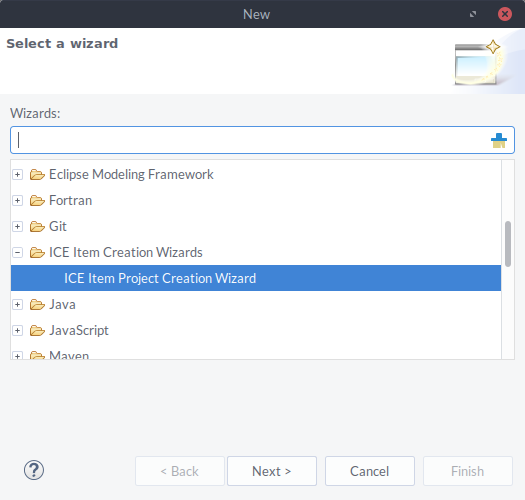
\includegraphics[width=8cm]{images/2}
\end{center}

To create a new ICE Item project click the \texttt{New} button in the left hand
side of the toolbar.  From the wizard that appears you should find a section
called \texttt{ICE Item Creation Wizards}; open this and select \texttt{ICE
Item Creation Wizard} and click the \texttt{Next >} button.

\begin{center}
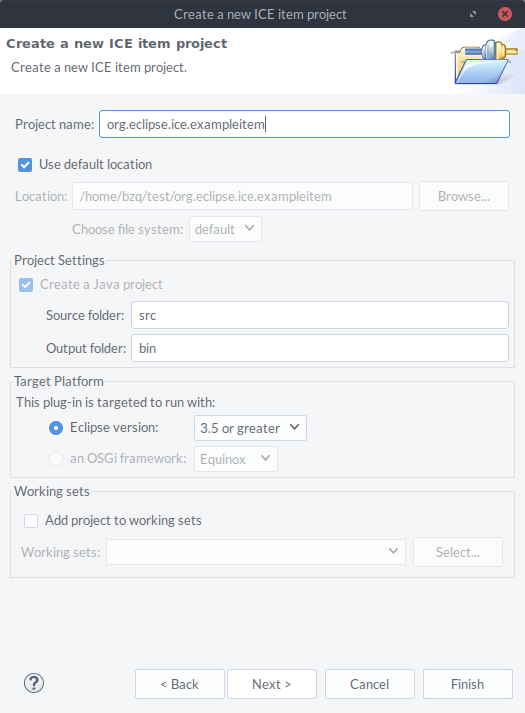
\includegraphics[width=8cm]{images/3}
\end{center}

You will be met with a standard new project wizard page, in which you can name
your project.  We will call ours \texttt{org.eclipse.ice.exampleitem}.  You do
not need to prefix your project with the \texttt{org.eclipse.ice} text, though
we do to showcase the packaging of the generated code.  Once you have named
your project click the \texttt{Next >} button.

\begin{center}
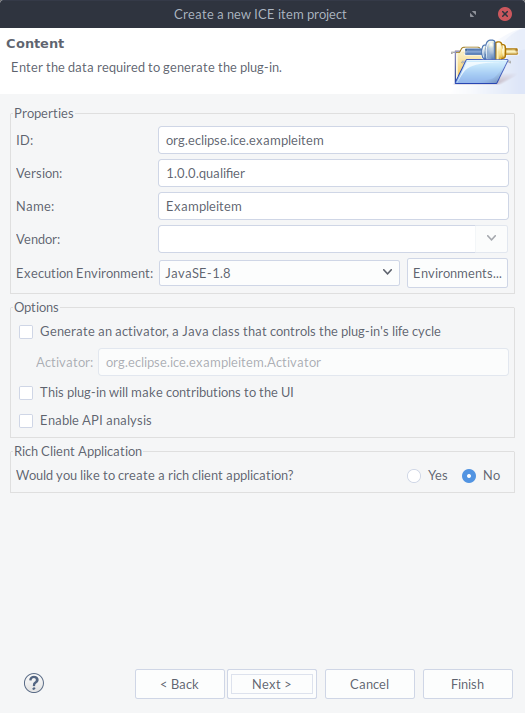
\includegraphics[width=8cm]{images/4}
\end{center}

Now you are able to customize the plugin-specific portions of the project.  You
do not need to do anything at the point unless you have specific requirements.
We will simply go to the next page by clicking the \texttt{Next >} button
again.

\begin{center}
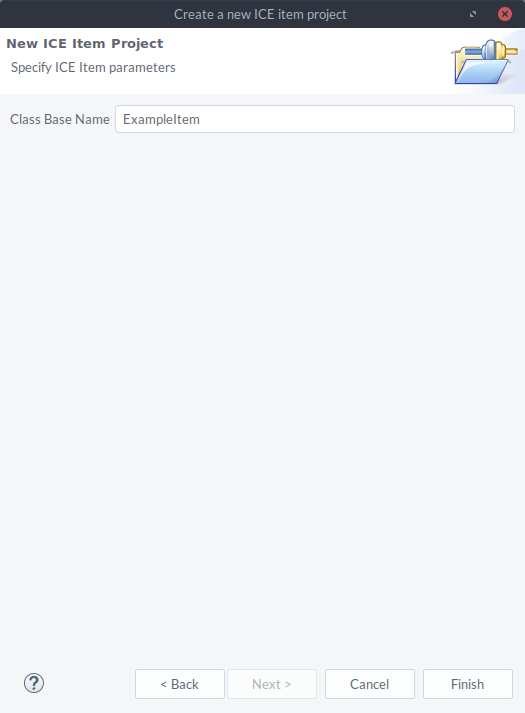
\includegraphics[width=8cm]{images/5}
\end{center}

On this page you will have to tell the wizard what you want to use as a base
name for your item classes.  We will call it \texttt{ExampleItem}, though you
could name it anything you want.  When you have entered your base class name
you can click the \texttt{Finish} button to generate your new item plugin
project.

\begin{center}
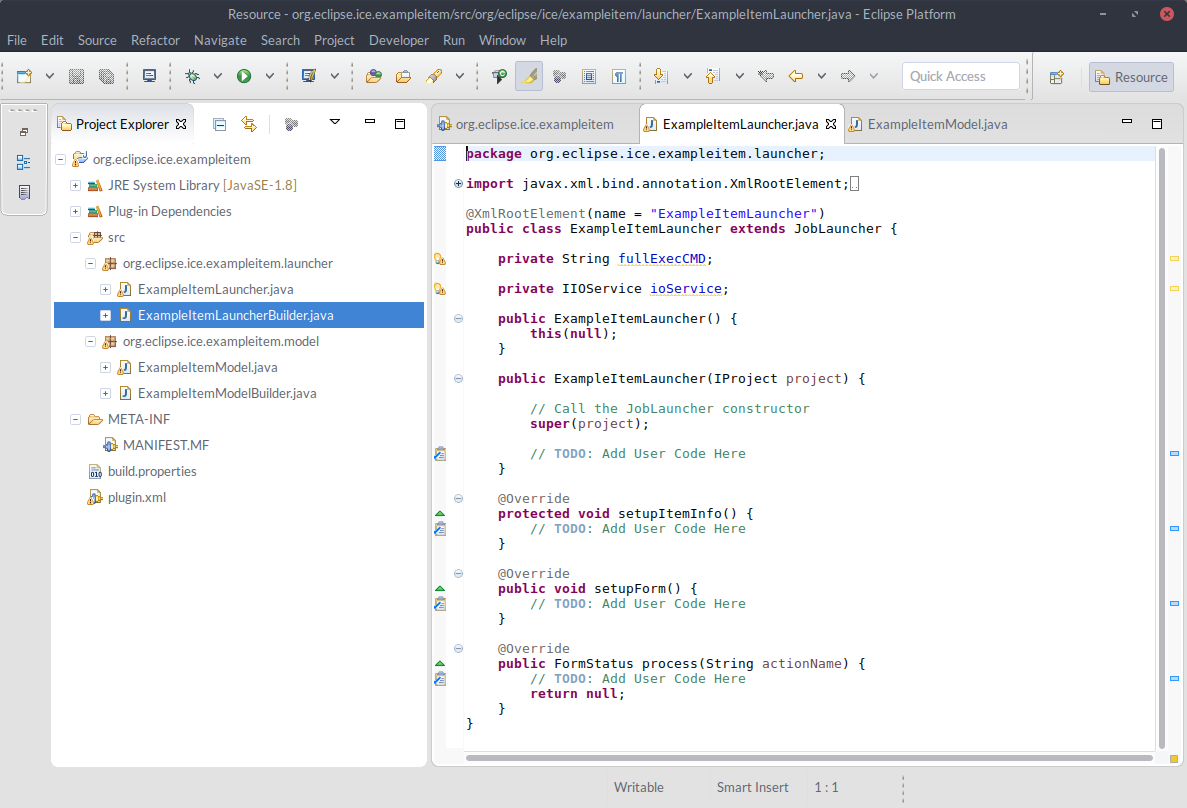
\includegraphics[width=12cm]{images/6}
\end{center}

When the project has finished generating you should be able to explore the code
that has been created.  Within the source directory there will be two packages,
each containing two Java classes:

\begin{itemize}
    \item \texttt{org.eclipse.ice.exampleitem.launcher}
    \begin{itemize}
        \item \texttt{ExampleItemLauncher.java}
        \item \texttt{ExampleItemLauncherBuilder.java}
    \end{itemize}
    \item \texttt{org.eclipse.ice.exampleitem.model}
    \begin{itemize}
        \item \texttt{ExampleItemModel.java}
        \item \texttt{ExampleItemModelBuilder.java}
    \end{itemize}
\end{itemize}

To add functionality to the project you will only be responsible for editing
the \texttt{Launcher} and \texttt{Model} classes and can ignore the
\texttt{LauncherBuilder} and \texttt{ModelBuilder} classes.

\section{Adding functionality to the project}


\section{Building and incorporating your item into ICE}


\end{document}

